\chapter{Introduction}
\section{The beginnings of microbiology and microbial ecology}
%
For centuries, humans have been curious to understand the unseen organisms that surround them: this is the basic objective of microbial ecology. Up until the 17th century, however, prominent scientists were naive to the lifeforms that could not be observed with the naked eye. The field of microscopy began to expand when the Englishman Robert Hooke developed one of the first compound microscopes and published the book \textit{Micrographia} \cite{Hooke1665} in 1665 with detailed drawings of never before observed images of magnified organisms and structures. It was in this book that he coined the term cell after observing plant cells from cork tissue. He based this term on the resemblance to the walled structure in honeycomb. Unfortunately, very little is known of Hooke's career and accomplishments (there does not even exist a portrait of him) due to his falling out with contemporary scientists of prominence, namely Sir Isaac Newton \cite{Espinasse1962}.	

Hooke's microscopy work inspired others, however. Antonie van Leeuwenhoek took an interest in Hooke's Micrographia in order to apply microscopy to his business of owning and operating a drapery \cite{Dobell1932}. Leeuwenhoek, a Dutch businessman, was intent to use the finest quality thread and fabric for his work, and believed he could have an advantage over his competitors if he were to use an instrument with higher magnification than modern magnifying glasses to inspect the material for imperfections. Leeuwenhoek was skilled at grinding lenses from glass and was able to craft microscopes with 200X magnification, thus surpassing the capability of the best microscopes at the time, the most powerful of which had 30X magnification. He began to discover many microscopic structures which had yet to be observed. Most notable among these observations were blood cells, sperm cells, and protists and algae from pond water. After he would record his observations, he would write letters in Dutch to the Royal Society of London, which would be translated to English or Latin and then published by the society. In 1683, Leeuwenhoek wrote a letter to the Royal Society detailing the life forms which he had observed within plaque sampled from between his teeth. He wrote of the motility and the dense occurrence of at least two types of ``animalcules'', what we now know as bacteria. These observations led to the emergence of the microbiology and microbial ecology fields.

\section{The foundation of modern microbial ecology experiments}
%
Microbial ecology is the broad study of microbial organisms in their natural environments \cite{Atlas1986}. One of the primary objectives of microbial ecology is to understand the complete diversity of microbial organisms cohabitating a single environment. This objective includes understanding the taxonomic classification of the detectable microbes. Culturing individual microbial isolates from environmental samples, which was established by Robert Koch in the late 19th century \cite{nobel1967}, was a promising technique for surveying the microorganisms present in each sample. However, it was found apparent that the diversity levels capable of being cultured on media were underwhelming compared to the diversity of microorganisms observed under a microscope. Specifically, in soil, <1\% of microorganisms are capable of being cultured under laboratory conditions \cite{Hugenholtz1998}. Thus culturing isolated microbes is currently a fruitless task for surveying overall diversity, while microscopy will give little to no answers about the taxonomic information of the observed microbes. 

In order to get a better grasp of the microorganisms present in environments and to what taxonomic classifications they belong, scientists turned to culture-independent surveys \cite{Hugenholtz1998}. One groundbreaking and seminal technique was the use of 16S ribosomal RNA to classify microorganisms phylogenetically by Carl Woese and colleagues. Woese, in the mid 1970's, was skeptical of the dogma that all organisms separate into 2 domains solely based on the presence or absence of a nucleus, i.e. eukaryotes and prokaryotes. In his seminal study \cite{Woese1977}, Woese complained that ``Dividing the living world into Prokaryotae and Eukaryotae has served, if anything, to obscure the problem of what extant groupings represent the various primeval branches from the common line of descent.'' He made this complaint because using presence or absence of nuclei as a classifier of domain is not a phylogenetic measure, and thus scientists cannot resolve evolutionary relationships in any meaningful way using this metric. Woese and his colleague, John Fox, proved their point by comparing 16S rRNA sequences found in prokaryotic microorganisms to 18S rRNA sequences from eukaryotes (the homologous eurkaryotic rRNA to 16S rRNA in prokaryotes) \cite{Woese1977}. They used 16S rRNA as the phylogenetic marker because they needed a biological molecule that was conserved across the tree of life, slowly evolved over time, and was easily extractable from cells. No known protein fit these descriptions at the time. They found that, through analysis of 16S rRNA, prokaryotic organisms had 2 distinct lineages which were similarly distant from each other as each lineage was to eukaryotes. They termed these lineages as eubacteria and archaebacteria. Not only did Woese and Fox discover a new domain of life, but they laid the groundwork for using the phylogenetically conserved 16S rRNA subunit as a marker for topologically describing the tree of life.

Woese conducted his fundamental studies on cultured organisms. Norman Pace, a colleague of Woese, began to apply 16S rRNA sequencing to unculturable organisms to identify evolutionary lineages of uncharacterized bacteria and archaea \cite{Pace1986}. The scientific community soon adopted his approach and the vast topology of the tree of life began to fill in. In the 1980's, when these studies were taking place, DNA sequencing was a tedious, non-trivial process. Two decades later, DNA sequencing technology reached major breakthroughs causing the rapid expansion of genomic studies and importantly microbial ecology studies.

\section{The rise in modern microbial ecology}
%
Relatively recently, the use of culture-independent techniques to study microbial community structure has been rebranded under new field names. The Google search terms ``microbiome'' and ``microbiota'' are trending over the last decade and are still rising. The search term for ``microbial ecology'', on the other hand, is decreasing. I will define the terms microbiome and microbiota and give a few potential reasons as to why these fields have expanded in popularity.

\begin{figure}[tbh]
\centering
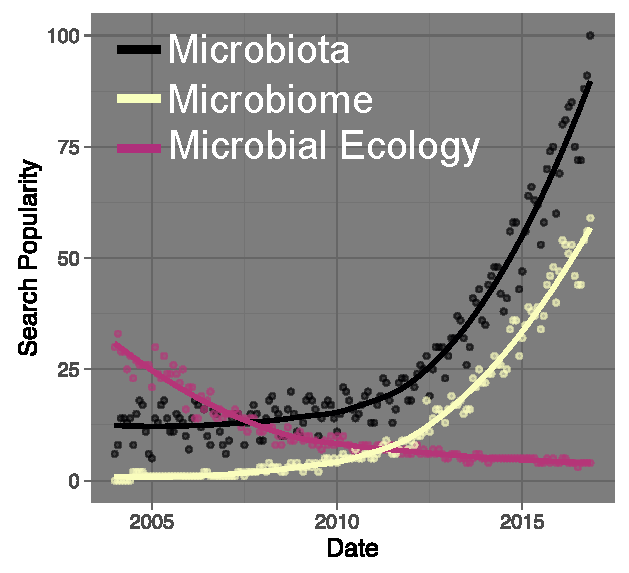
\includegraphics[width=2.75in]{Figures/intro_fig1}
% where an .eps filename suffix will be assumed under latex,
% and a .pdf suffix will be assumed for pdflatex
\caption[Figure 1.1]{Popularity of Google searches for terms related to microbial ecology over the last decade. Data was collected from Google Trends (https://www.google.com/trends/).}
\label{Figure 1.1}
\end{figure}

A microbiota is the complete catalog of microorganisms inhabiting an environment. The definition of the environment can range depending on the study system, but typically the term microbiota refers to microbial communities that are associated with a multicellular host. Many researchers use the term microbiome and microbiota interchangeably; however, some researchers define the microbiome as the complete genomic content of the microbiota. For the sake of this dissertation, I will use the terms ``microbiome'' and ``microbiota'' synonymously. The study of the human gut microbiota by Jeffrey Gordon's lab has led to growing interests in host-associated microbiota. Peter Turnbaugh, Ruth Ley and Fredrik Backhed, all members of Gordon's Laboratory, drew a direct connection between the gut microbiota and the host species' physiology and phenotype \cite{Turnbaugh,Backhed,Ley2005}. They showed that lean and obese mice hosted significantly different communities of microbes in their guts and when an obese mouse gut microbiota was inoculated into lean mice or germ free mice (i.e. mice that have no microbes in their gut) that the recipients rapidly gained body fat. These studies definitively showed that the gene content of the microbiota residing in the gut of a host animal, has the ability to significantly influence the physiology and health of the host. These studies were instrumental for initiating the Human Microbiome Project \cite{Turnbaugh2007} as well as providing a significant motivation for studying all other host-associated microbiomes, including plant microbiomes.

\begin{figure}[tbh]
\centering
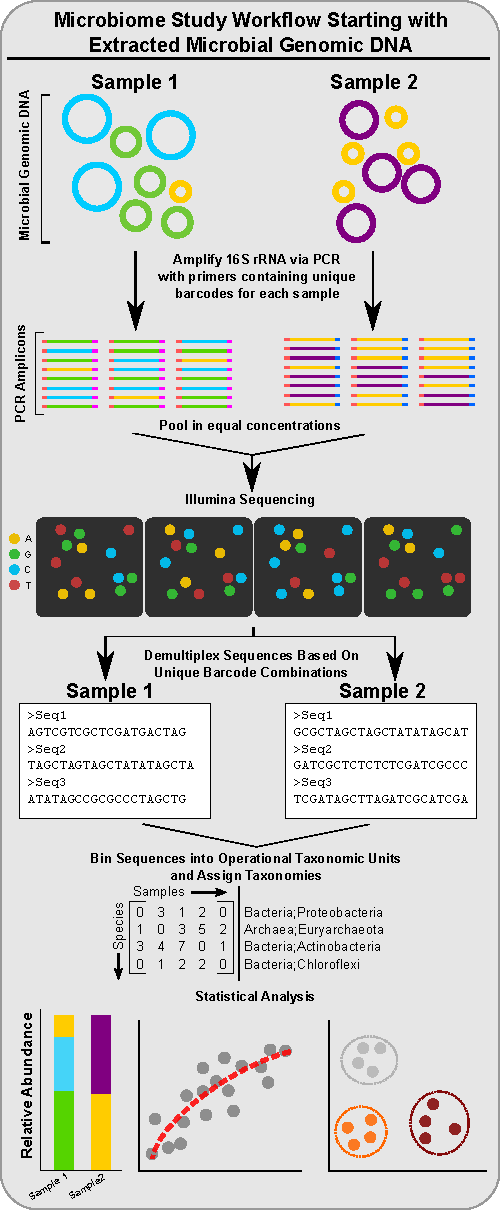
\includegraphics[width=2.75in]{Figures/intro_fig2}
% where an .eps filename suffix will be assumed under latex,
% and a .pdf suffix will be assumed for pdflatex
\caption[Figure 1.2]{Standard workflow for profiling microbial communities from environmental DNA.}
\label{Figure 1.2}
\end{figure}

While biological advances drew a considerable amount of interest to the field of microbiomes, sequencing capability still posed technical barriers for understanding host-associated microbial communities in depth. 16S rRNA sequencing was the method of choice for profiling microbial communities but researchers were burdened by the process of cloning 16S rRNA PCR amplicons into plasmids, cloning into Escherichia coli, and using Sanger sequencing to survey microbial diversity within samples. This method is relatively tedious, very low throughput, and expensive. At the time, a standard study would profile 300-400 different clones for each sample. Next generation sequencing again revolutionized the technical aspect of microbial ecology field. The first application of pyrosequencing to 16S rRNA sequencing was by Sogin et al in 2006 \cite{Sogin2006}. They were able to sequence over 119,000 16S rRNA sequence tags and importantly they were able to barcode separate samples into a single sequencing run. Pyrosequencing became the preferred method for researchers investigating microbiomes, but this technology would soon be surpassed. Illumina sequencing, which had previously not been applicable to profiling 16S rRNA fragments due to read length limitations, began to emerge as the standard method for sequencing once the MiSeq platform was introduced in 2011 \cite{Caporaso2011}. Compared to the previous iteration of Illumina chemistry, the MiSeq platform allowed for greater read lengths, while maintaining the high throughput standard with Illumina. The general workflow for community profiling using 16S rRNA gene sequencing is shown in Figure 1.2.

\section{Plant Associated Microbiomes}
%
The impact of host-associated microbial communities on animal health is a robust area of research. Investigators are similarly interested in plant-associated microbiota. As sessile organisms, plants rely on their environment for the uptake of critical nutrients \cite{Epstein1971}. Co-habitating the soil with plants are thousands of different bacterial and archaeal strains, some of which are known to aid host plants in tolerating otherwise inhospitable conditions. For example, the genus Lupinus in the Fabaceae family, thrives in nitrogen poor soil where other plants struggle to survive. The lupine received its name because it was thought to act as a wolf, plundering nutrients in the soil and thus making the environment unfavorable for the growth of other plants \cite{Austin2004}. This hypothesis was false. In fact, lupines and other members of the Fabaceae family, form symbiotic relationships with nitrogen fixing soil bacteria thereby allowing them to survive otherwise nitrogen limited conditions \cite{Vance2001}. This is an important and widespread example of how plants form beneficial relationships with soil microbes.
	
Plants also rely on soil microbes to survive attacks from pathogens \cite{Berendsen2012,Bulgarelli2012}. In some cropping systems, such as sugar beet and wheat, continuous monoculture cultivation of soil leads to reduced loss of yield from pathogen infection \cite{Hornby1983}. It was found that this phenomenon is transmissible to other, non-suppressive soils and that the effect is lost upon pasteurization at $80\,^{\circ}\mathrm{C}$, thus suggesting that the mechanism is biological in nature \cite{Hornby1983}. Mendes et al. tested the root-associated bacterial communities between sugar beet seedlings grown in soils suppressive to \textit{Rhizoctonia solani} infection and soils conducive for infection (sampled from the margin of the fields where suppressive soils were located) \cite{Mendes2011}. They found that no single bacterial or archaeal strain was responsible for the difference in microbial community structure between suppressive and conducive soils. Many of the microbial strains they detected differed in relative abundance between the soils, mainly within the Gamma and Beta Proteobacterial classes. These results were instrumental in demonstrating how broader microbial communities, i.e. the root microbiota, are important for soil and plant health.

Because soil microbial communities were found to impact plant health, deep characterizations of the plant root microbiota began to take place. In 2012, two groups published studies characterizing the root-associated microbiota of \textit{Arabidopsis thaliana} \cite{Bulgarelli2012,Lundberg2012,}. These studies found that the consortia of microbes inside of the root (the endosphere) is significantly different and of lower diversity than the microbial communities in the soil adhering to the root (the rhizosphere). Each study found that variability in microbial community structure between different soils is also reflected in the root-associated microbial assemblages of the plants grown in the respective soils. The studies found plant genotype to have a small but significant effect on the microbial communities associated with the roots. It was later found in rice that there is a third discernible niche on the rhizoplane (the root surface) and that these microbial communities are intermediate in composition between the rhizosphere and endosphere \cite{Edwards2015}. A longitudinal study of early microbiome acquisition in rice detailed the dynamic changes in microbiota composition within the rhizosphere, rhizoplane, and endosphere compartments \cite{Edwards2015}. Together this data suggested a three-step model that we proposed \cite{Edwards2015} for microbiota assembly in the root: microbes are first attracted to the roots in the rhizosphere, perhaps by root exudates, after which a select set of microbes can attach to the rhizoplane and a subset of rhizoplane attached microbes can enter the root endosphere.

Open questions still remain for the plant root-associated microbiota. Functionally, there are only limited examples of how root associated bacterial and archaeal communities may impact plant fitness. Further studies are needed to assess how the root-associated microbiota may aid plants in tolerating abiotic and biotic stresses. Once a better understanding of how microbiomes may help to protect plants from various stresses is attained, researchers are intent to leverage crop genetics to breed for beneficial root microbiotas. Because intraspecies genetic variation has a minimal impact on the root-associated microbiota, it is of importance to better understand how host interspecies variation impacts the root-associated microbiome and what physiological traits are causal of microbiome divergence between plant species. It is also critical to understand how root associated microbial communities change over the life cycle of the host plant. Plants face different nutritional requirements at various stages of their lives, but it is yet to be characterized how root-associated microbial communities shift over the growing season and how these potential changes are tied to plant developmental shifts. 

In this disseration, I characterize various aspects of the root-associated microbiome of the crop plant rice. Rice is an important model for studying plant-microbe interactions for several reasons: rice displays a unique growth habit for crop plants by growing in submerged anaerobic soils, rice is a contributor to greenhouse gas emissions \cite{Minami1994} (a process mediated by soil microbes), and is also in need of a yield boost to feed the world's growing population, perhaps by breeding for latent traits \cite{khush2005will}. This disseration is separated into three research chapters. In the first chapter, I characterize the root-associated microbiota of rice plants and quantify the factors affecting root assemblages. In the second chapter, I characterize how the rice root microbiota differs from other crop species as well as how the rice root microbiota differs from native plants growing in the same flooded environment. In this chapter I also show how continuous and intensive cultivation of rice enriches for a soil microbiota with rice specific microbes. In the final chapter, I demonstrate the dynamics of the root-associated microbiota over the life cycle of the rice plant and how the abundances of specific microbial taxa are tuned by the developmental stage of the host plant.